\documentclass{beamer}
\usetheme{afm}

\title{Modeling Correlation \\ \vspace{0.25cm} between Risks}
\author{Matteo Sani - \href{mailto:matteo.sani@unisi.it}{matteo.sani@unisi.it}}

\begin{document}
\begin{frame}[plain]
	\maketitle
\end{frame}

\begin{frame}{Distribution Transformation}
  \begin{itemize}
  \item Distribution transformation (also called \emph{inverse transform} or \emph{percentile-to-percentile transform}) is used to transform a random variable PDF to a uniform distribution and vice versa.
  \item The key ingredient of this method are:
    \begin{enumerate}
      \item computing the CDF or the quantile function of a distribution;
      \item uniform samples can be interpreted as cumulative probabilities (i.e.  CDF$_{\textrm{uniform}}(X)=X$).
    \end{enumerate}
  \end{itemize}

  \begin{equation*}
    \begin{gathered}
      \textrm{uniform\_sample} \rightarrow \tt{distribution.ppf(uniform\_sample)} \rightarrow \textrm{distribution\_sample}\\
      \textrm{distribution\_sample} \rightarrow \tt{distribution.cdf(distribution\_sample)} \rightarrow \textrm{uniform\_sample}
    \end{gathered}
  \end{equation*}
\end{frame}

\begin{frame}{Distribution Transformation}
  \begin{figure}[h]
    \begin{center}
    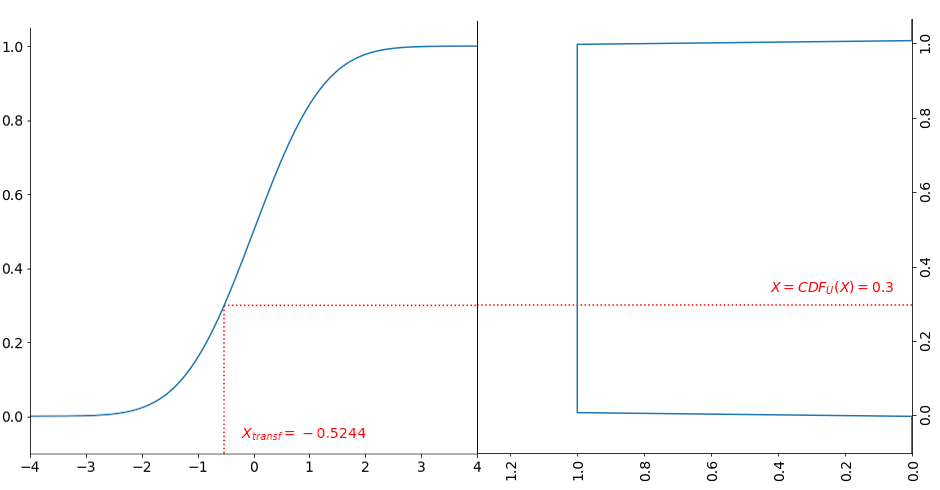
\includegraphics[width=0.7\linewidth]{ppf_transform}
    \end{center}
  \end{figure}    
\end{frame}

\begin{frame}[fragile]{Example}
  $U(X)$ is the uniform distribution: to convert to normal just apply the quantile function (the inverse of the CDF).
  \begin{ipython}
from scipy.stats import norm

U = [0.3, 0.5, 0.9, 0.999999999]

for x in U:
    print (f"{x} => {norm.ppf(x))}")
  \end{ipython}
\begin{ioutput}
0.3 => -0.5244005127080409
0.5 => 0.0
0.9 => 1.2815515655446004
0.999999999 => 5.997807019601637
\end{ioutput}
\end{frame}
	
\begin{frame}[fragile]{Example with \texttt{numpy}}
  \begin{columns}
    \column{0.5\linewidth}
    \begin{itemize}	
    \item $\tt{python}$ provides an easier way to apply such transformations:
    \item  Given a distribution class (e.g. \texttt{uniform}, \texttt{norm},...):
      \begin{itemize}
      \item \texttt{rvs(size=1000)} method samples \texttt{size=1000} times from it;
      \item methods like \texttt{cdf} or \texttt{ppf} take in input \texttt{numpy.array},  a particular kind of list, \emph{allowing to avoid loop-cycles}: the transformation itself is indeed automatically applied to each item of the array.
      \end{itemize}
    \end{itemize}
    \column{0.5\linewidth}
\tiny{
    \begin{ipython}
from scipy.stats import uniform, norm
import numpy as np, time

N = 10000
x_unif = uniform.rvs(size=N)

# standard: slower, more code
t1 = time.time()
x = np.empty(N)
for i in range(len(x_unif)):
  x[i] = norm.ppf(x_unif[i])
print ("Method 1: ", time.time() - t1)

# "vectorization": ~ x300 faster
t2 = time.time()
x = norm.ppf(x_unif)
print("Method 2: ", time.time() - t2)      
\end{ipython}
\begin{ioutput}
Method 1: 2.312714099884033
Method 2: 0.0075719356536865234
\end{ioutput}
    }
    \end{columns}
\end{frame}

\begin{frame}{What's Happening ?}
  \begin{itemize}
  \item With a 2D plot we can get a sense of what is going on when using the inverse CDF transformation
    \begin{figure}[h]
      \begin{center}
        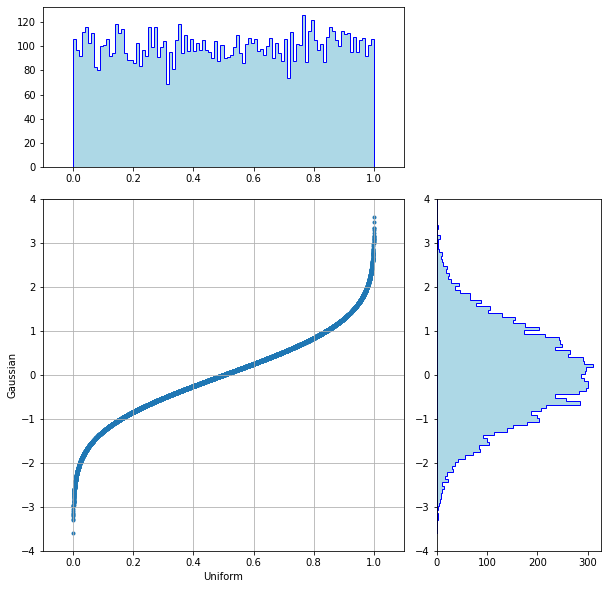
\includegraphics[width=0.4\linewidth]{uniform_to_gauss_2d}
      \end{center}
    \end{figure}    
  \item The transformation stretches the outer regions of the uniform to yield a normal distribution. 
  \item This technique can be used with any arbitrary (univariate) probability distributions, like for example t-Student or Gumbel.
  \end{itemize}
\end{frame}

\begin{frame}[fragile]{From Arbitrary Distribution to Uniform}
  To go from an arbitrary distribution to uniform, just apply the inverse of the inverse CDF, which is the CDF itself\ldots
  \begin{figure}[h]
    \begin{center}
      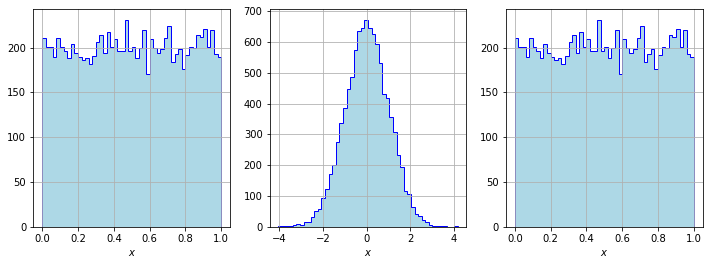
\includegraphics[width=0.7\linewidth]{full_chain}
    \end{center}
  \end{figure}
  \begin{ipython}
from scipy.stats import norm, uniform

x_unif = uniform.rvs(size=10000)
x2 = norm.ppf(x_unif)
x3 = norm.cdf(x2)
\end{ipython} 
\end{frame}

\begin{frame}{Copula}
  \begin{itemize}
  \item In general \emph{correlation measures the tendency of two or more companies to "influence" their behavior}. 
  \item The estimate of default probabilities and their correlations is the most important issue in credit derivative valuation and credit risk management. 
  \item The estimate through \emph{historical default data} is very inaccurate (low default data availability, inadequacy of data...); so \emph{mathematical models} are used.
  \item \emph{Copulas} are used to describe dependencies between random variables related with risk. 
  \item A copula $\mathcal{C}(F_1, F_2, \ldots, F_n)$ is a multivariate cumulative distribution function whose marginal probability distributions (the probability distribution of each dimension) are uniform. 
  \item Very popular since allows to easily model and estimate the distribution of random vectors by representing marginal distributions and their correlation separately: \emph{a complicated problem can be split into simpler components}.
  \end{itemize}
\end{frame}

\begin{frame}[fragile]{Example}
\begin{itemize}
	\item Image you have modelled the seasonal water level of a river and the flood probability of the same river.
	\begin{figure}[h]
		\begin{center}
		    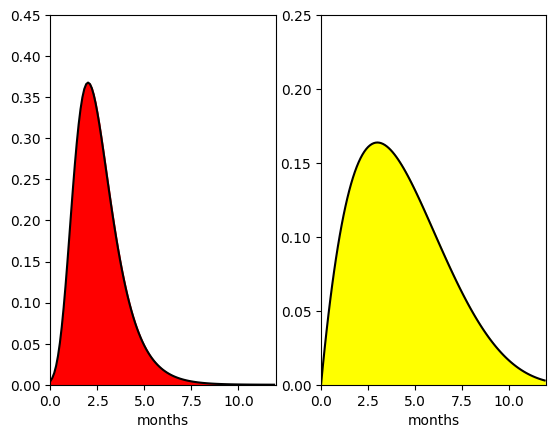
\includegraphics[width=0.4\linewidth]{floods}
		\end{center}
	\end{figure}
	\item Clearly the two distributions are correlated, i.e. the higher the level of water the higher the flood probability.
	\item How can we express the joint distribution to be able to answer a question like "what is the probability to have a flood given the river is at $X~m$ ?". 
\end{itemize}
\end{frame}

%\begin{frame}[fragile]{Example}
%  Consider the daily returns of BMW and Siemens stocks $(2010-2022)$, \href{https:\/\/github.com\/matteosan1\/finance\_course\/raw\/develop\/input\_files\/bmw\_siemens.csv}{bmw\_siemens.csv}.
%  \begin{ipython}
%import pandas as pd
%
%data = pd.read_csv("bmw_siemens.csv", index_col="Date")
%
%bmw = data.loc[:, 'BMW.DE']
%sie = data.loc[:, 'SIE.DE']
%
%print (data[['BMW.DE', 'SIE.DE']].corr())
%\end{ipython}
%  \begin{ioutput}
%          BMW.DE    SIE.DE
%BMW.DE  1.000000  0.664654
%SIE.DE  0.664654  1.000000    
%\end{ioutput}
%\end{frame}
%
%\begin{frame}{Example}
%  \begin{itemize}
%    \item \emph{It's reasonable to assume that the returns of the two are correlated}: same country and similar sector.
%    \item Imagine you want to model the joint distribution of their returns to know what is the probability both shares go negative at the same time.
%    \item \emph{Copula} can simplify the model (the joint probability distribution) by splitting it into marginals (by definition no correlation) and a function which \emph{couples} them together.
%    \item By fitting the historical histograms we can determine the marginal distributions (t-student).
%  \end{itemize}
% \begin{figure}[h]
%   \begin{center}
%     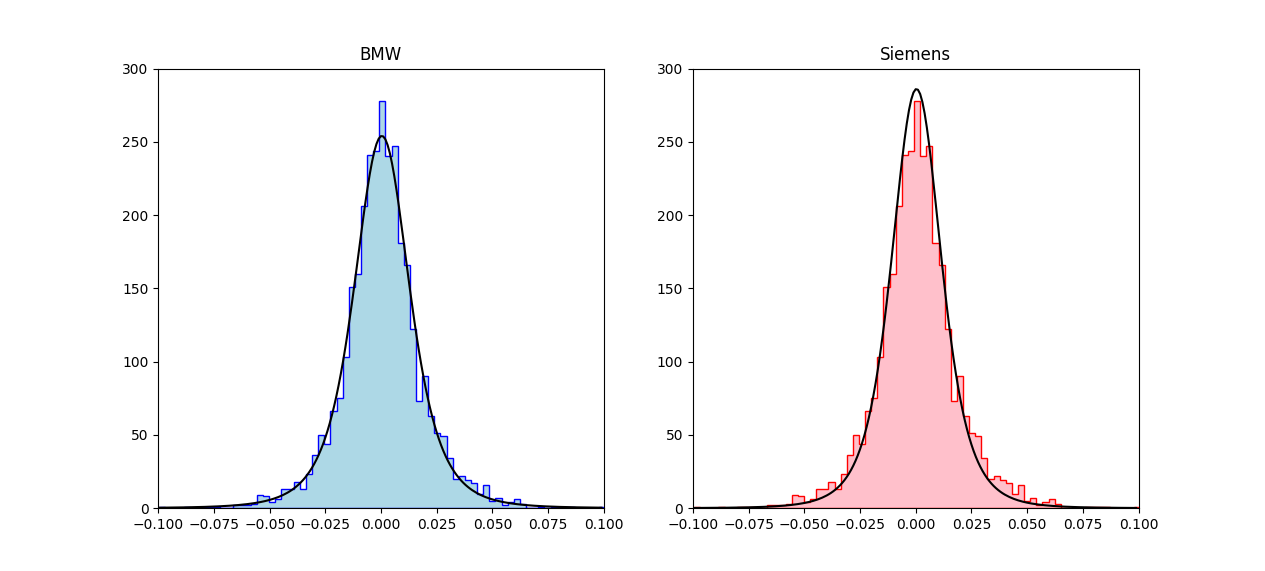
\includegraphics[width=0.65\linewidth]{bmw_siemens_dist}
%   \end{center}
% \end{figure}
%\end{frame}
%
%\begin{frame}[fragile]{Modeling Correlation with Copulas (1)}
%  Sample from a \emph{multivariate normal} (2D) with a 0.66 correlation (the covariance matrix is $
%      \Sigma = \begin{bmatrix}
%        \sigma^2 (X_0) & \mathrm{Cov}(X_0, X_1)\\
%        \mathrm{Cov}(X_1, X_0) & \sigma^2 (X_1)
%      \end{bmatrix}$
%  \begin{columns}
%    \column{0.65\linewidth}
%    \begin{ipython}
%from scipy.stats import multivariate_normal
%import numpy as np
%      
%np.random.seed(1)
%N = 100000
%mv = multivariate_normal(mean=[0,0],
%         cov=data[['BMW.DE', 'SIE.DE']].corr())
%x = mv.rvs(size=N)
%\end{ipython}
%\column{0.35\linewidth}
%  \begin{figure}[h]
%    \begin{center}
%      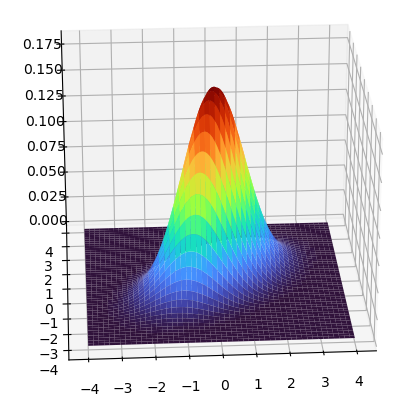
\includegraphics[width=0.9\linewidth]{3d_gauss_corr}
%    \end{center}
%  \end{figure}
%  \end{columns}
%\end{frame}
%
%\begin{frame}[fragile]{Modeling Correlation with Copulas (2)}
%  Now transform the marginals to uniform using the \texttt{cdf} method. 
%  \begin{ipython}
%from scipy.stats import norm
%
%copula = norm.cdf(x)    
%\end{ipython}
%  \begin{figure}[h]
%    \begin{center}
%      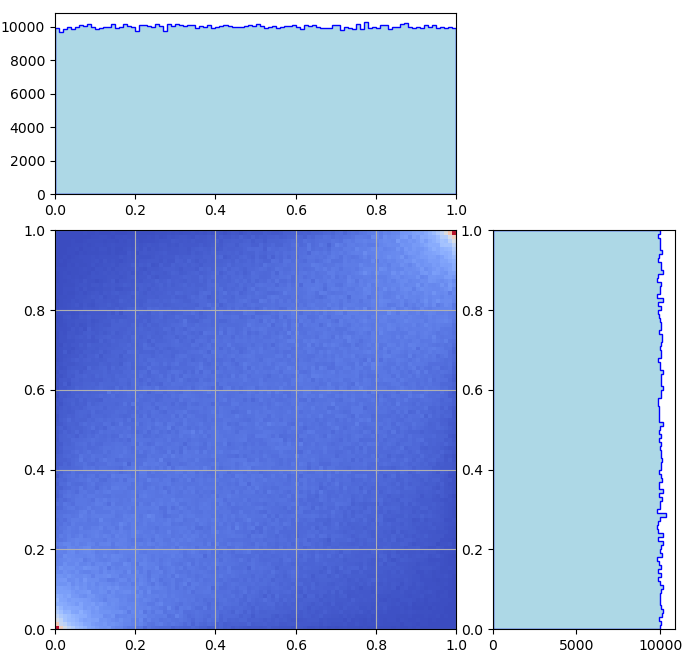
\includegraphics[width=0.4\linewidth]{copula_2d} \quad
%      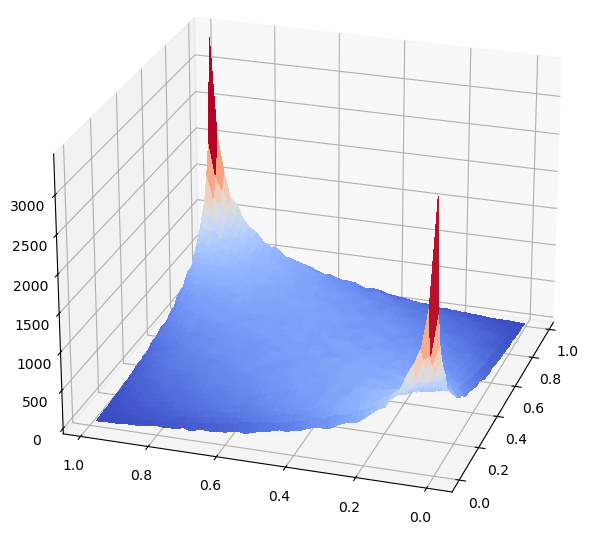
\includegraphics[width=0.4\linewidth]{copula_3d}
%    \end{center}
%  \end{figure}
%  \emph{Since we used a multivariate standard normal to model correlation this is also called a Gaussian Copula.}
%\end{frame}
%
%\begin{frame}[fragile]{Modeling Correlation with Copulas (3)}
% Finally we can just transform the marginals from uniform to what we want (i.e. the two t-students in our example):
%\begin{ipython}
%from scipy.stats import t
%
%bmw_fit = t.fit(bmw[1:])
%sie_fit = t.fit(sie[1:])
%
%bmw_f = t(*bmw_fit)
%sie_f = t(df=sie_fit[0], loc=sie_fit[1], scale=sie_fit[2])
%
%# convert uniform marginals with fitted functions
%bmw_corr = bmw_f.ppf(copula[:, 0])
%sie_corr = sie_f.ppf(copula[:, 1])
%
%# uncorrelated
%bmw_uncorr = bmw_f.rvs(size=100000)
%sie_uncorr = sie_f.rvs(size=100000)
%\end{ipython}
%\end{frame}
%
%\begin{frame}[fragile]{Results}
%  Now that we have a model for the joint distribution of the share returns we can compute the probability to have both of them negative.
%  \begin{ipython}
%# correlated
%n1, n2, N = 0, 0, 100000 
%for i in range(N):
%  if bmw_corr[i] < 0 and sie_corr[i] < 0:
%    n1 += 1
%  if bmw_uncorr[i] < 0 and sie_uncorr[i] < 0:
%    n2 += 1
%
%print ("corr: ", n1/N)
%print ("uncorr: ", n2/N)
%\end{ipython}
%\begin{ioutput}
%corr: 0.353726
%uncorr: 0.23536
%\end{ioutput}
%\end{frame}

\begin{frame}[fragile]{Results}
  \begin{figure}[h]
    \begin{center}
      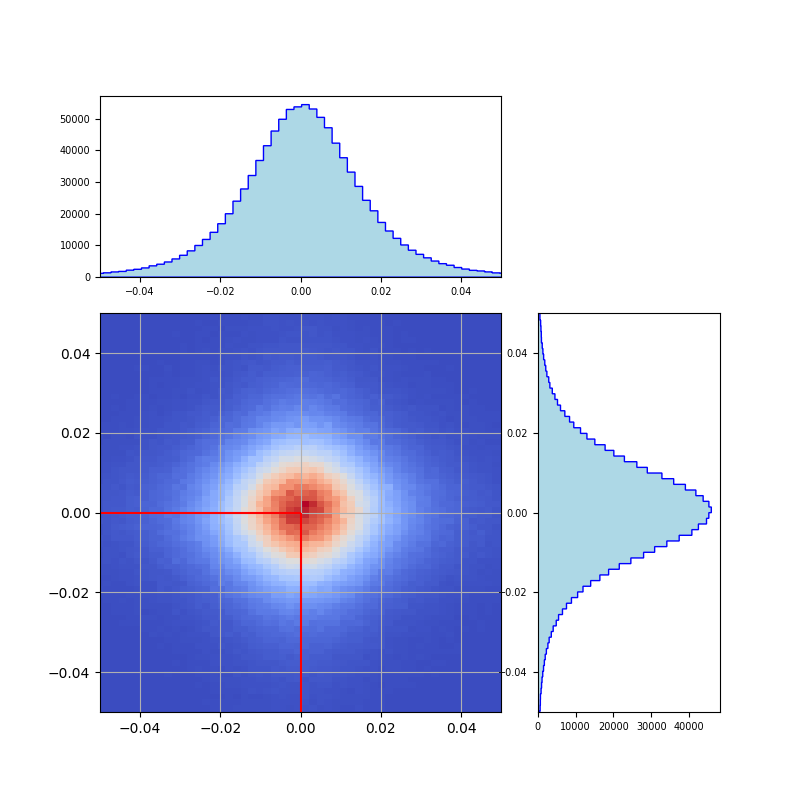
\includegraphics[width=0.45\linewidth]{bmw_siemens_corr} \quad
      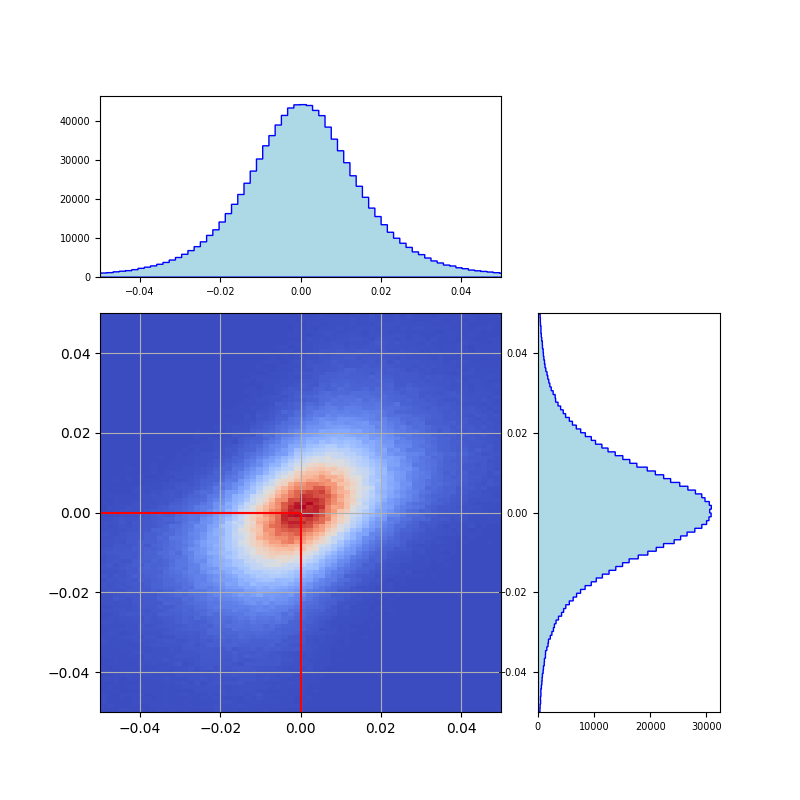
\includegraphics[width=0.45\linewidth]{bmw_siemens_uncorr}
    \end{center}
  \end{figure}
\end{frame}

\begin{frame}{Remark}
  \emph{"Extreme, synchronized rises and falls in financial markets occur
infrequently but they do occur. The problem with the models is that
they did not assign a high enough chance of occurrence to the scenario
in which many things go wrong at the same time the “perfect storm” scenario"}.
  \begin{figure}[h]
    \begin{center}
      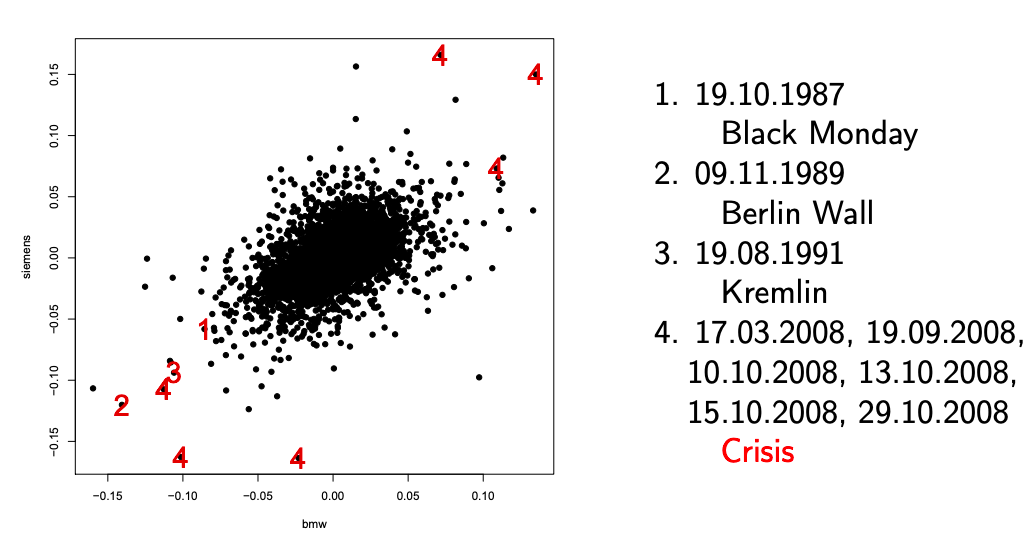
\includegraphics[width=0.7\linewidth]{crisis}
    \end{center}
  \end{figure}
\end{frame}

\begin{frame}{Remark}
Gaussian copula is nice and easy to construct but tends to underestimate events on the tails. So it is often used the \emph{t-student copula} which has fatter tails but preserves the same (bell shaped, non-skewed) characteristics of the Gaussian.

\begin{figure}[h]
  \begin{center}
    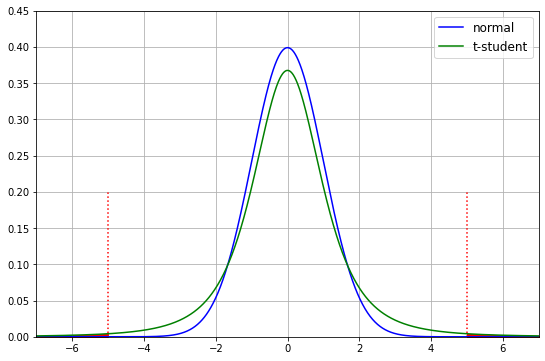
\includegraphics[width=0.5\linewidth]{gauss_vs_t}
  \end{center}
\end{figure}
\end{frame}

\begin{frame}[fragile]{Remark}
\begin{itemize}
	\item We can estimate the \emph{frequency} of a highly improbable event (i.e. $5\sigma$) in the two cases.
	\item If $P_{5\sigma}$ is the probability, $1/P_{5\sigma}$ is \emph{the number of times the event "fails" for every time it succeeds}, e.g $P_{5\sigma}=0.5$, the event would happen every 2 days for example.
	\item Since we are interested in very good AND very bad events:
	$P_{5\sigma} = F(X\leq-5\sigma) + F(X\geq5\sigma) = 2\cdot F(X\leq-5\sigma)$, with $F$ the CDF of symmetric distribution. 
\end{itemize}
 \begin{ipython}
from scipy.stats import norm, t

freq_g = 1/(norm.cdf(-5)*2)/365
freq_t = 1/(t(4.1, 0, 1).cdf(-5)*2)/30

print (f"Once every {freq_g:.0f} years")
print (f"Once every {freq_t:.1f} months")
\end{ipython}
\begin{ioutput}
Once every 4779 years
Once every 4.7 months
\end{ioutput}
\end{frame}

\begin{frame}{Basket Default Swap}
  \begin{itemize}
  \item A basket default swap (BDS) is a credit derivative on a portfolio of n reference entities:
    \begin{itemize}
      \item the simplest basket default swaps are first-to-default, second-to-default, \ldots, nth-to-default swaps. 
    \end{itemize}
  \item Very similar to normal CDS except for the protection they offer:
    \begin{itemize}
      \item a first-to-default swap provides insurance for only the first default happening;
      \item a second-to-default swap provides insurance for only the second default\ldots
    \end{itemize}
  \item For example, in a nth-to-default swap, the seller does not make any payment to the protection buyer for the first $n-1$ defaulted entities, and makes it only for the $n^{th}$ default. Once there has been this payment the swap terminates.
  \end{itemize}
\end{frame}

\begin{frame}{n$^{th}$-to-default Basket Valuation}
  \begin{itemize}
  \item Assume the principals and expected recovery rates are the same for all underlying reference assets, also all the assets have the same default probability.
  \item The valuation procedure is similar to that for a regular CDS:
    \begin{itemize}
    \item in CDS depends on $P_d$ of the reference asset between times $t_1$ and $t_2$;
    \item in BDS depends on $P_d$ that the $n^{th}$ asset default was between times $t_1$ and $t_2$.
    \end{itemize}
  \item The buyer of protection makes quarterly payments at a specified rate until the $n^{th}$ default occurs or the end of the life of the contract is reached. 
  \item In the event of the $n^{th}$ default occurring, the seller pays $F\cdot(1-R)$.
  \end{itemize}
\end{frame}

\end{document}

